\section{Experiments in the four-dimensional case}
\noindent Let us examine the four-dimensional case. While the generalization of the problem to four dimensions is quite straightforward, the treatment of it is noticeably more difficult than that of lower dimensions. This is not only due to the greatly increased search space and subtle challenges in discarding symmetries. The real challenge arises from the fact that a RDTS must contain more than one dimension tuple. However, it took a long time to realize this and in order to get started, it was necessary to make a number of decisions, where the most appropriate choice was not obvious, simply because of the sparse knowledge of this problem.

Initially it seemed natural that examining any dimension tuple satisfying Hoffman's inequality and with distinct elements would represent the ``most difficult'' case. This is the line of thought presented by Spiridonov in \cite[p. 6]{Spiridonov_2003} and, after all, the immediate generalization of Hoffman's focus in \cite[p. 215]{Hoffman1981}. However, when attempting to count the number of four-dimensional squares it became clear that the number depended on the concrete choice of dimension tuple (satisfying Hoffman's inequality and with distinct elements). \cref{fig:4d-squares-good-bad} gives an example of a square without overlap for one of these dimension tuples, but with overlap for a different one.
\begin{figure}[ht]
    \centering
    \begin{subfigure}[b]{0.47\textwidth}
        \centering
            \begin{tikzpicture}[scale=0.12]
                \filldraw[fill=custom-red, draw=black] (0,0) rectangle (8,9);
\filldraw[fill=custom-blue, draw=black] (0,9) rectangle (12,17);
\filldraw[fill=custom-violet, draw=black] (0,17) rectangle (12,27);
\filldraw[fill=custom-yellow, draw=black] (0,27) rectangle (9,39);
\filldraw[fill=custom-blue, draw=black] (8,0) rectangle (20,8);
\filldraw[fill=custom-red, draw=black] (12,8) rectangle (20,17);
\filldraw[fill=custom-green, draw=black] (12,17) rectangle (20,27);
\filldraw[fill=custom-violet, draw=black] (9,27) rectangle (19,39);
\filldraw[fill=custom-yellow, draw=black] (20,0) rectangle (29,12);
\filldraw[fill=custom-red, draw=black] (20,12) rectangle (29,20);
\filldraw[fill=custom-orange, draw=black] (20,20) rectangle (29,30);
\filldraw[fill=custom-yellow, draw=black] (19,30) rectangle (31,39);
\filldraw[fill=custom-green, draw=black] (29,0) rectangle (39,8);
\filldraw[fill=custom-orange, draw=black] (29,8) rectangle (39,17);
\filldraw[fill=custom-violet, draw=black] (29,17) rectangle (39,29);
\filldraw[fill=custom-green, draw=black] (31,29) rectangle (39,39);
            \end{tikzpicture}
        \caption{Square of $\paren{8, 9, 10, 12}$ without overlap.}
    \end{subfigure}
    ~
    \begin{subfigure}[b]{0.47\textwidth}
        \centering
            \begin{tikzpicture}[scale=0.12*39/49]
                \filldraw[fill=custom-red, draw=black] (0,0) rectangle (10,12);
\filldraw[fill=custom-blue, draw=black] (0,12) rectangle (14,22);
\filldraw[fill=custom-violet, draw=black] (0,22) rectangle (14,35);
\filldraw[fill=custom-yellow, draw=black] (0,35) rectangle (12,49);
\filldraw[fill=custom-blue, draw=black] (10,0) rectangle (24,10);
\filldraw[fill=custom-red, draw=black] (14,10) rectangle (24,22);
\filldraw[fill=custom-green, draw=black] (14,22) rectangle (24,35);
\filldraw[fill=custom-violet, draw=black] (12,35) rectangle (25,49);
\filldraw[fill=custom-yellow, draw=black] (24,0) rectangle (36,14);
\filldraw[fill=custom-red, draw=black] (24,14) rectangle (36,24);
\filldraw[fill=custom-orange, draw=black] (24,24) rectangle (36,37);
\filldraw[fill=custom-yellow, draw=black] (25,37) rectangle (39,49);
\filldraw[fill=custom-green, draw=black] (36,0) rectangle (49,10);
\filldraw[fill=custom-orange, draw=black] (36,10) rectangle (49,22);
\filldraw[fill=custom-violet, draw=black] (36,22) rectangle (49,36);
\filldraw[fill=custom-green, draw=black] (39,36) rectangle (49,49);
            \end{tikzpicture}
        \caption{Square of $\paren{10, 12, 13, 14}$ with overlap.}
    \end{subfigure}
    \caption{Example of the same square produced using two different dimension tuples. Using the second dimension tuple produces an overlap.}
    \label{fig:4d-squares-good-bad}
\end{figure}
This sudden overlap is due to a reliance on a non-trivial overlap inequality. Hence, it seemed appropriate to choose to completely exclude a partial solution if there is a pair of hyperrectangles where it relies solely on non-trivial overlap inequality to prevent overlap. This posed a problem, since---as we will see shortly---a four-dimensional dimension tuple will always satisfy at least one non-trivial overlap inequality. Hence, it was no longer possible to search for universal packings using a concrete dimension tuple, and this complicated the search considerably. However, this choice was later challenged by the discovery of a universal packing relying solely on non-trivial overlap inequalities for some of its overlap comparisons. It turns out that some non-trivial inequalities must be satisfied when others are not.
\begin{figure}[ht]
    \centering
    \begin{subfigure}[b]{0.47\textwidth}
        \centering
            \begin{tikzpicture}[scale=0.12]
                \filldraw[fill=custom-violet, draw=black] (0,0) rectangle (12,10);
\filldraw[fill=custom-orange, draw=black] (0,10) rectangle (12,19);
\filldraw[fill=custom-violet, draw=black] (0,19) rectangle (10,31);
\filldraw[fill=custom-blue, draw=black] (0,31) rectangle (10,39);
\filldraw[fill=custom-blue, draw=black] (12,0) rectangle (20,10);
\filldraw[fill=custom-red, draw=black] (12,10) rectangle (20,19);
\filldraw[fill=custom-orange, draw=black] (10,19) rectangle (19,31);
\filldraw[fill=custom-red, draw=black] (10,31) rectangle (19,39);
\filldraw[fill=custom-violet, draw=black] (20,0) rectangle (30,12);
\filldraw[fill=custom-blue, draw=black] (20,12) rectangle (30,20);
\filldraw[fill=custom-violet, draw=black] (19,20) rectangle (31,30);
\filldraw[fill=custom-orange, draw=black] (19,30) rectangle (31,39);
\filldraw[fill=custom-orange, draw=black] (30,0) rectangle (39,12);
\filldraw[fill=custom-red, draw=black] (30,12) rectangle (39,20);
\filldraw[fill=custom-blue, draw=black] (31,20) rectangle (39,30);
\filldraw[fill=custom-red, draw=black] (31,30) rectangle (39,39);
            \end{tikzpicture}
        \caption{Square of $\paren{8, 9, 10, 12}$.}
    \end{subfigure}
    ~
    \begin{subfigure}[b]{0.47\textwidth}
        \centering
            \begin{tikzpicture}[scale=0.12*39/49]
                \filldraw[fill=custom-violet, draw=black] (0,0) rectangle (14,13);
\filldraw[fill=custom-orange, draw=black] (0,13) rectangle (14,25);
\filldraw[fill=custom-violet, draw=black] (0,25) rectangle (13,39);
\filldraw[fill=custom-blue, draw=black] (0,39) rectangle (13,49);
\filldraw[fill=custom-blue, draw=black] (14,0) rectangle (24,13);
\filldraw[fill=custom-red, draw=black] (14,13) rectangle (24,25);
\filldraw[fill=custom-orange, draw=black] (13,25) rectangle (25,39);
\filldraw[fill=custom-red, draw=black] (13,39) rectangle (25,49);
\filldraw[fill=custom-violet, draw=black] (24,0) rectangle (37,14);
\filldraw[fill=custom-blue, draw=black] (24,14) rectangle (37,24);
\filldraw[fill=custom-violet, draw=black] (25,24) rectangle (39,37);
\filldraw[fill=custom-orange, draw=black] (25,37) rectangle (39,49);
\filldraw[fill=custom-orange, draw=black] (37,0) rectangle (49,14);
\filldraw[fill=custom-red, draw=black] (37,14) rectangle (49,24);
\filldraw[fill=custom-blue, draw=black] (39,24) rectangle (49,37);
\filldraw[fill=custom-red, draw=black] (39,37) rectangle (49,49);
            \end{tikzpicture}
        \caption{Square of $\paren{10, 12, 13, 14}$.}
    \end{subfigure}
    \caption{Example of square without overlap produced using two dimension tuples which satisfy different non-trivial overlap inequalities. This is surprising since the square relies on non-trivial overlap inequalities to prevent overlap.}
    \label{fig:4d-square-universal}
\end{figure}
\cref{fig:4d-square-universal} illustrates an effect of this phenomenon. Here there are no overlaps in either of the two squares, but for some pairs of hyperrectangle this is due to a gap along one dimension in the first square and a different dimension in the second square. This discovery is the true motivation behind introducing the notion of a RDTS and the elaborate machinery surrounding it.

\begin{example}[RDTS for $n = 4$]\label[example]{ex:4d-rdts}
In this case all overlap inequalities have arity $1$, $2$ or $3$. By \cref{prop:arity-reduction} we only have to consider the overlap inequalities with arity $1$ or $2$. We would like to choose a dimension tuple $\paren{x_1, x_2, x_3, x_4}$ satisfying Hoffman's inequality and containing distinct elements. Of the overlap inequalities with arity $1$, such a dimension tuple will only satisfy the trivial ones. If this is possible, then we only need to consider the overlap inequalities with arity $2$. Suppose $\paren{A, B}$ is a non-trivial overlap inequality with arity $2$. If $A \cap B \neq \emptyset$, then the inequality is really a non-trivial overlap inequality of arity $1$ in disguise by \cref{lemma:arity-minus-common-terms}. If $A \cap B = \emptyset$, then the only possibilities are
\[
x_1 + x_4 \leq x_2 + x_3 \quad
x_2 + x_3 \leq x_1 + x_4 \quad
x_2 + x_4 \leq x_1 + x_3
\quad \text{and} \quad
x_3 + x_4 \leq x_1 + x_2.
\]
However, if we choose dimension tuples with distinct elements, then the last two will not be satisfied. Thus, we are left with
\[
x_1 + x_4 \leq x_2 + x_3
\quad \text{and} \quad
x_2 + x_3 \leq x_1 + x_4.
\]
Observe that if one is not satisfied, then the other must be satisfied. However, it depends on the concrete choice of dimension tuple, whether only the first, only the second or both of them are satisfied. Observe that $d_1 = \paren{8, 9, 10, 12}$ and $d_2 = \paren{10, 12, 13, 14}$ both satisfy Hoffman's inequality and both contain distinct elements. Notice that $d_1$ does not satisfy the first overlap inequality, since $8 + 12 > 9 + 10$, while $d_2$ does not satisfy the second, since $12 + 13 > 10 + 14$. Hence $[d_1]$ and $[d_2]$ are the minimal elements and by \cref{prop:minimal-rdts}
\[
T = \curly{\paren{8, 9, 10, 12}, \paren{10, 12, 13, 14}}
\]
is a RDTS for $n = 4$. Intuitively, we have covered every possible way that we can linearly order the sums of two distinct terms (without any two sums with different terms being equal). This is illustrated in \cref{fig:hasse-4d-arity-2}.
\end{example}

\begin{figure}[ht]
    \centering
    \begin{subfigure}[b]{0.4\textwidth}
        \centering
            \begin{tikzpicture}[scale=1]
                \node (12) at (0,0) {$\curly{1, 2}$};
                \node (13) at (0,1) {$\curly{1, 3}$};
                \node (23) at (1,2) {$\curly{2, 3}$};
                \node (14) at (-1,2) {$\curly{1, 4}$};
                \node (24) at (0,3) {$\curly{2, 4}$};
                \node (34) at (0,4) {$\curly{3, 4}$};
                \draw (12) -- (13) -- (23) -- (24)
                      (13) -- (14) -- (24) -- (34);
                \draw [semithick, custom-red, dotted] (23) -- (14);
            \end{tikzpicture}
        \caption{The four-dimensional case.}
        \label{fig:hasse-4d-arity-2}
    \end{subfigure}
    ~
    \begin{subfigure}[b]{0.4\textwidth}
        \centering
            \begin{tikzpicture}[scale=1]
                \node (12) at (0,0) {$\curly{1, 2}$};
                \node (13) at (0,1) {$\curly{1, 3}$};
                \node (23) at (1,2) {$\curly{2, 3}$};
                \node (14) at (-1,2) {$\curly{1, 4}$};
                \node (24) at (1,3) {$\curly{2, 4}$};
                \node (15) at (-1,3) {$\curly{1, 5}$};
                \node (34) at (1,4) {$\curly{3, 4}$};
                \node (25) at (-1,4) {$\curly{2, 5}$};
                \node (35) at (0,5) {$\curly{3, 5}$};
                \node (45) at (0,6) {$\curly{4, 5}$};
                \draw (12) -- (13) -- (23) -- (24) -- (34) -- (35) -- (45)
                      (13) -- (14) -- (15) -- (25) -- (35)
                      (14) -- (24) -- (25);
                \draw [semithick, custom-red, dotted] (14) -- (23) -- (15) -- (34) -- (25)
                               (24) -- (15);
            \end{tikzpicture}
        \caption{The five-dimensional case.}
        \label{fig:hasse-5d-arity-2}
    \end{subfigure}
    \caption{Hasse diagrams of the partial ordering of sums with two distinct terms. Dotted lines represent relations which can not be determined in general. Each set $\curly{i, j}$ can by thought of as the sum $x_i + x_j$.}
\end{figure}

\begin{remark}\label[remark]{remark:bad-4d-tuple}
Spiridonov considers the dimension tuple $d = \paren{99, 100, 101, 102}$, because ``the sizes differ by a very small amount'' \cite[p. 6]{Spiridonov_2003}. Notice that $d$ satisfies both of the non-trivial overlap inequalities above as
$99 + 102 = 100 + 101$. Hence, if Spiridonov were to find a Hoffman packing of $d$, it might not produce a packing of neither $d_1$ nor $d_2$ in the example above. In particular, it might not be a universal packing.
\end{remark}

\subsection{Utilizing approaches from the three-dimensional case}
\noindent Let us begin by considering the dynamic programming approach.

\subsubsection{Dynamic programming}
We have used the dynamic programming approach to construct all squares in the four-dimensional case using the same strategy as in the three-dimensional case, that is by first constructing all lines and then combining them into squares. Note that this time a square is not automatically specialized as it was in the three-dimensional case.

\begin{observation}\label[observation]{obs:4d-dynamic-programming}
There are $4! = 24$ possible lines and if we specify one more dimension there are $24 \cdot 3^4 = 1\,944$. Using dynamic programming we have determined that there are $S = 51\,247\,458$ squares of the RDTS from \cref{ex:4d-rdts} without overlaps and satisfying the Line criterion \labelcref{criterion:line-criterion}. Observe that our count is different from---and quite a bit lower---than the $77\,436\,138$ squares counted by Spiridonov \cite[p. 6]{Spiridonov_2003} using the dimension tuple, which we questioned the choice of in \cref{remark:bad-4d-tuple}. We have reproduced his results for that choice of dimension tuple, but we still maintain that $S$ is the appropriate number due to its independence of the choice of dimension tuple.
\end{observation}

\noindent It takes a few minutes to generate all of the squares in the four-dimensional case and as we will see below, constructing all cubes does not seem to be practically possible for now. Let us attempt to estimate the number of cubes in the four-dimensional case and the computations needed to determine the exact number, if we construct them by stacking four squares. We only consider the consequences of the Line criterion \labelcref{criterion:line-criterion}, since it is difficult to predict overlap.

First, let us consider how many ways we can specialize the $4^2 = 16$ rectangles in a single square. There are two choices for each one, giving $2^{16}$ possible specializations. Hence, letting $S$ be defined as in \cref{obs:4d-dynamic-programming} there are $2^{16} S$ ways to choose the first square. Next, we would like to stack a second specialized square on top of it. For simplicity and due to the inclusion of symmetries we suppose that there is a $3/4$ probability that the heights of two bricks on top of each other will be different, so we estimate around $(3/4)^{16} 2^{16} S$ specialized squares to be compatible with the first choice. Hence, we estimate there to be around $(3/4)^{16} 2^{32} S^2 = 3^{16} S^2$ half-cubes. At his point, the half-cubes are presumably so constrained by the Line criterion \labelcref{criterion:line-criterion} that we consider an estimate of the number of compatible squares for the third square as too much guesswork. However, we can classify the half-cubes into $6^{16}$ groups depending on the $\binom{4}{2} = 6$ different ways to choose the brick heights in each of the $16$ stacks of two bricks. Under the assumption that the half-cubes distribute evenly into these groups, we estimate that one can exhaust the search space by checking
\[
\paren{3^{16} S^2}^2 6^{-16} \approx 4.5 \cdot 10^{33}
\]
different combinations of four squares. It is difficult to predict how many of these will have overlapping bricks. We have found $U = 1\,119\,514\,176$ different squares satisfying the Line criterion \labelcref{criterion:line-criterion}, if we do not check for overlaps while only $S/U \approx 4.58\%$ are in fact without overlapping bricks. Since there are more possibilities for overlaps in a cube, we suspect the actual number of cubes without overlapping bricks to be several orders of magnitude lower, but still quite large.

Next, let us consider the backtracking approach where we have been able to relatively quickly find a cube in the four-dimensional case.

\subsubsection{Backtracking}
We have tried out the procedures described in \cref{table:backtracking-procedures}, but it has not been possible to find a solution within a reasonable time frame. However, each of the procedures finds a cube satisfying the Subgrid criterion \labelcref{criterion:subgrid-criterion} in around a minute. This gives us a basis for comparing the different procedures. Again, procedure D is a notable improvement over the naive procedure A requiring 84\% fewer iterations to find a cube. The details can be found in \cref{table:backtracking-3d}. This improvement and the significance of the different criteria is illustrated in \cref{fig:backtracking-4d}. Notice that the detection of sharp corners (procedure B) gives the most significant improvement as opposed to checking the Subgrid criterion \labelcref{criterion:subgrid-criterion} (procedure C), while it was the other way around in the three-dimensional case.
\begin{table}[ht]
\centering
\caption{Number of iterations needed to find a cube satisfying the Subgrid criterion \labelcref{criterion:subgrid-criterion} in the four-dimensional case depending on the different test procedures.}
\label{table:backtracking-cubes-4d}
\bgroup
\def\arraystretch{1.1}
\begin{tabular}{|l|c|c|c|c|}
\hline
Procedure  & A  & B & C & D \\ \hline
First cube  & $209\,073\,771$ & $44\,589\,896$ & $169\,640\,571$ & $33\,419\,146$ \\ \hline
\end{tabular}
\egroup
\end{table}

\begin{figure}[ht]
    \centering
    \begin{tikzpicture}
        \begin{axis}[
            height=0.7\textwidth,
            width=\textwidth,
            xmin=0, xmax=220000000,
            ymin=0, ymax=70,
            scaled x ticks=false,
            x tick label style = {
                rotate=45,
                anchor=north east
            },
            xlabel=Iteration,
            ylabel=Number of hyperrectangles placed,
            grid=both,
            legend style={at={(0.99,0.018)},
            anchor=south east
            }
        ]
        
            \addplot+[
                draw=custom-red,
                mark=none,
                mark last,
                mark options={
                    scale=1,
                    fill=custom-red
                }
            ]
            table[x index=0, y index=2]{data/backtrack-4d-simple.dat};
            \addlegendentry{Procedure A}
            
            \addplot+[
                draw=custom-green,
                mark=none,
                mark last,
                mark options={
                    scale=1,
                    fill=custom-green
                }
            ]
            table[x index=0, y index=2]{data/backtrack-4d-corners.dat};
            \addlegendentry{Procedure B}
            
            \addplot+[
                draw=custom-blue,
                mark=none,
                mark last,
                mark options={
                    scale=1,
                    fill=custom-blue
                }
            ]
            table[x index=0, y index=2]{data/backtrack-4d-subspaces.dat};
            \addlegendentry{Procedure C}
            
            \addplot+[
                draw=custom-orange,
                mark=none,
                mark last,
                mark options={
                    scale=1,
                    fill=custom-orange
                }
            ]
            table[x index=0, y index=2]{data/backtrack-4d-corners-subspaces.dat};
            \addlegendentry{Procedure D}
        \end{axis}
    \end{tikzpicture}
    \caption{Plot of the number of hyperrectangles placed after a certain number of iterations in the four-dimensional case depending on the different test procedures. Here, we terminate as soon as a cube with $4^3 = 64$ bricks satisfying the Subgrid criterion \labelcref{criterion:subgrid-criterion} is found.}
    \label{fig:backtracking-4d}
\end{figure}
\begin{figure}[ht]
    \centering
    \begin{tikzpicture}
        \begin{axis}[
            height=0.7\textwidth,
            width=\textwidth,
            xmin=0, xmax=146600000000,
            ymin=0, ymax=120,
            scaled x ticks=false,
            x tick label style = {
                rotate=45,
                anchor=north east
            },
            xlabel=Iteration,
            ylabel=Number of hyperrectangles placed,
            grid=both,
            legend style={at={(0.99,0.018)},
            anchor=south east}
        ]
        
            \addplot+[
                draw=custom-red,
                mark=none,
                name path=A
            ]
            table[x index=0, y index=1]{data/backtrack-4d-best.dat};
            \addlegendentry{Fewest}
            
            \addplot+[
                draw=custom-green,
                mark=none
            ]
            table[x index=0, y index=2]{data/backtrack-4d-best.dat};
            \addlegendentry{Current}
            
            \addplot+[
                draw=custom-blue,
                mark=none,
                name path=B
            ]
            table[x index=0, y index=3]{data/backtrack-4d-best.dat};
            \addlegendentry{Most}
            %\addplot[custom-orange] fill between[of=A and B];
        \end{axis}
    \end{tikzpicture}
    \caption{Plot of the number of hyperrectangles placed after a certain number of iterations in the four-dimensional case using procedure D. The number of hyperrectangles have been sampled every $10^8$ iterations, each time noting the current number of hyperrectangles placed as well as the fewest and the most hyperrectangles having been placed since the previous sample was taken.}
    \label{fig:backtracking-4d-best}
\end{figure}
Using backtracking with procedure D for several days does not increase our hope of finding a solution. As shown in \cref{fig:backtracking-4d-best} the approach appears to be stuck at around 86 hyperrectangles placed. Hence, these two approaches does---at least in their current form---not show much promise of finding a solution in the four-dimensional case within a reasonable time frame. However, before proceeding any further, we present the following observation, which we referred to earlier.

\begin{observation}\label[observation]{obs:4d-universal-counterexamples}
In the four-dimensional case using backtracking it is possible to generate a large number of cubes within a few hours. After doing so we obtained over $900\,000$ cubes and selected a sample of 900 of these. We have investigated whether a cube in this sample produces a valid subpacking of increasing dimension tuples not necessarily satisfying Hoffman's inequality. It turns out that every cube from the sample produces a valid subpacking of any increasing dimension tuple $\paren{x_1, x_2, x_3, x_4}$ with integer values $1 \leq x_1 \leq x_2 \leq x_3 \leq x_4 \leq 100$.
\end{observation}

\subsection{Counting the number of unique squares}
We can still determine the number of unique squares and as a by-product also provide some interesting insights into exploiting the wish to ignore symmetries. Using either backtracking or dynamic programming, one can obtain the number of squares including symmetries in a few minutes. One would suspect this number---which we know to be $S = 51\,247\,458$ from \cref{obs:4d-dynamic-programming}---to be divisible by $2!\cdot 2^2 = 8$, since each square has $8$ symmetries. However, $8$ does not divide $S$, so something does not add up. Let us investigate this discrepancy.

It turns out that since four is an even dimension, we can in fact come across squares where some symmetries coincide. A way to approach discarding symmetries is to try and mimic the concept of a ``middle'' brick, which we have in odd dimensions. We do so by considering the hyperrectangles around the ``middle''. We will refer to this group as a \textit{kernel}\index{Kernel}. A kernel consists of 4 rectangles in the case of a square in the four-dimensional case. Observe that if two squares are a symmetry of one another, then their kernels must be as well. Thus, suppose we compute all possible kernels and discard their symmetries. Then a square obtained by completing one kernel can never be a symmetry of the completion of a different kernel. This divides the search into smaller parts which can be solved independently. However, we are not completely done with the trickiness of symmetries. If a kernel has 8 distinct symmetries, i.e.\ none of them coincide, then any two different completions to a square can not be a symmetry of each other. However, for a kernel where some of its symmetries coincide, then any two different completions of it could potentially be a symmetry of one another. If this is the case we need to discard one of them.

\begin{observation}
We have found that there are $6\,564$ square kernels not violating the Line criterion \labelcref{criterion:line-criterion} in the four-dimensional case. Notice that this number is not divisible by $8$, so some of the kernels must have coinciding symmetries. There are 6 kernels, which have only 2 distinct symmetries and these can be seen in \cref{fig:4d-square-self-two-symmetric-kernels}.

\begin{figure}[ht]
    \centering
    \begin{subfigure}[b]{0.14\textwidth}
        \centering
        \begin{tikzpicture}[scale=0.07]
            \filldraw[fill=custom-red, draw=black] (11,10) rectangle (19,19);
\filldraw[fill=custom-red, draw=black] (10,19) rectangle (19,27);
\filldraw[fill=custom-red, draw=black] (19,11) rectangle (28,19);
\filldraw[fill=custom-red, draw=black] (19,19) rectangle (27,28);
        \end{tikzpicture}
    \end{subfigure}
    ~
    \begin{subfigure}[b]{0.14\textwidth}
        \centering
        \begin{tikzpicture}[scale=0.07]
            \filldraw[fill=custom-green, draw=black] (11,9) rectangle (19,19);
\filldraw[fill=custom-green, draw=black] (9,19) rectangle (19,27);
\filldraw[fill=custom-green, draw=black] (19,11) rectangle (29,19);
\filldraw[fill=custom-green, draw=black] (19,19) rectangle (27,29);
        \end{tikzpicture}
    \end{subfigure}
    ~
    \begin{subfigure}[b]{0.14\textwidth}
        \centering
        \begin{tikzpicture}[scale=0.07]
            \filldraw[fill=custom-blue, draw=black] (11,7) rectangle (19,19);
\filldraw[fill=custom-blue, draw=black] (7,19) rectangle (19,27);
\filldraw[fill=custom-blue, draw=black] (19,11) rectangle (31,19);
\filldraw[fill=custom-blue, draw=black] (19,19) rectangle (27,31);
        \end{tikzpicture}
    \end{subfigure}
    ~
    \begin{subfigure}[b]{0.14\textwidth}
        \centering
        \begin{tikzpicture}[scale=0.07]
            \filldraw[fill=custom-orange, draw=black] (10,9) rectangle (19,19);
\filldraw[fill=custom-orange, draw=black] (9,19) rectangle (19,28);
\filldraw[fill=custom-orange, draw=black] (19,10) rectangle (29,19);
\filldraw[fill=custom-orange, draw=black] (19,19) rectangle (28,29);
        \end{tikzpicture}
    \end{subfigure}
    ~
    \begin{subfigure}[b]{0.14\textwidth}
        \centering
        \begin{tikzpicture}[scale=0.07]
            \filldraw[fill=custom-yellow, draw=black] (10,7) rectangle (19,19);
\filldraw[fill=custom-yellow, draw=black] (7,19) rectangle (19,28);
\filldraw[fill=custom-yellow, draw=black] (19,10) rectangle (31,19);
\filldraw[fill=custom-yellow, draw=black] (19,19) rectangle (28,31);
        \end{tikzpicture}
    \end{subfigure}
    ~
    \begin{subfigure}[b]{0.14\textwidth}
        \centering
        \begin{tikzpicture}[scale=0.07]
            \filldraw[fill=custom-violet, draw=black] (9,7) rectangle (19,19);
\filldraw[fill=custom-violet, draw=black] (7,19) rectangle (19,29);
\filldraw[fill=custom-violet, draw=black] (19,9) rectangle (31,19);
\filldraw[fill=custom-violet, draw=black] (19,19) rectangle (29,31);
        \end{tikzpicture}
    \end{subfigure}
    \caption{Square kernels in the four-dimensional case which have only 2 distinct symmetries.}
    \label{fig:4d-square-self-two-symmetric-kernels}
\end{figure}

Such a kernel consists of 4 of the same type of rectangle and the only distinct symmetry is obtained by a reflection. There are 18 kernels, which have only 4 distinct symmetries and these can be seen in \cref{fig:4d-square-self-four-symmetric-kernels}.

\begin{figure}[ht]
    \centering
    \begin{subfigure}[b]{0.14\textwidth}
        \centering
        \begin{tikzpicture}[scale=0.07]
            \filldraw[fill=custom-red, draw=black] (11,10) rectangle (19,19);
\filldraw[fill=custom-orange, draw=black] (10,19) rectangle (19,29);
\filldraw[fill=custom-orange, draw=black] (19,9) rectangle (28,19);
\filldraw[fill=custom-red, draw=black] (19,19) rectangle (27,28);
        \end{tikzpicture}
    \end{subfigure}
    ~
    \begin{subfigure}[b]{0.14\textwidth}
        \centering
        \begin{tikzpicture}[scale=0.07]
            \filldraw[fill=custom-red, draw=black] (11,10) rectangle (19,19);
\filldraw[fill=custom-yellow, draw=black] (10,19) rectangle (19,31);
\filldraw[fill=custom-yellow, draw=black] (19,7) rectangle (28,19);
\filldraw[fill=custom-red, draw=black] (19,19) rectangle (27,28);
        \end{tikzpicture}
    \end{subfigure}
    ~
    \begin{subfigure}[b]{0.14\textwidth}
        \centering
        \begin{tikzpicture}[scale=0.07]
            \filldraw[fill=custom-red, draw=black] (11,10) rectangle (19,19);
\filldraw[fill=custom-green, draw=black] (9,19) rectangle (19,27);
\filldraw[fill=custom-green, draw=black] (19,11) rectangle (29,19);
\filldraw[fill=custom-red, draw=black] (19,19) rectangle (27,28);
        \end{tikzpicture}
    \end{subfigure}
    ~
    \begin{subfigure}[b]{0.14\textwidth}
        \centering
        \begin{tikzpicture}[scale=0.07]
            \filldraw[fill=custom-red, draw=black] (11,10) rectangle (19,19);
\filldraw[fill=custom-violet, draw=black] (9,19) rectangle (19,31);
\filldraw[fill=custom-violet, draw=black] (19,7) rectangle (29,19);
\filldraw[fill=custom-red, draw=black] (19,19) rectangle (27,28);
        \end{tikzpicture}
    \end{subfigure}
    ~
    \begin{subfigure}[b]{0.14\textwidth}
        \centering
        \begin{tikzpicture}[scale=0.07]
            \filldraw[fill=custom-red, draw=black] (11,10) rectangle (19,19);
\filldraw[fill=custom-blue, draw=black] (7,19) rectangle (19,27);
\filldraw[fill=custom-blue, draw=black] (19,11) rectangle (31,19);
\filldraw[fill=custom-red, draw=black] (19,19) rectangle (27,28);
        \end{tikzpicture}
    \end{subfigure}
    ~
    \begin{subfigure}[b]{0.14\textwidth}
        \centering
        \begin{tikzpicture}[scale=0.07]
            \filldraw[fill=custom-red, draw=black] (11,10) rectangle (19,19);
\filldraw[fill=custom-violet, draw=black] (7,19) rectangle (19,29);
\filldraw[fill=custom-violet, draw=black] (19,9) rectangle (31,19);
\filldraw[fill=custom-red, draw=black] (19,19) rectangle (27,28);
        \end{tikzpicture}
    \end{subfigure}
    \par\bigskip
    \begin{subfigure}[b]{0.14\textwidth}
        \centering
        \begin{tikzpicture}[scale=0.07]
            \filldraw[fill=custom-green, draw=black] (11,9) rectangle (19,19);
\filldraw[fill=custom-yellow, draw=black] (10,19) rectangle (19,31);
\filldraw[fill=custom-yellow, draw=black] (19,7) rectangle (28,19);
\filldraw[fill=custom-green, draw=black] (19,19) rectangle (27,29);
        \end{tikzpicture}
    \end{subfigure}
    ~
    \begin{subfigure}[b]{0.14\textwidth}
        \centering
        \begin{tikzpicture}[scale=0.07]
            \filldraw[fill=custom-green, draw=black] (11,9) rectangle (19,19);
\filldraw[fill=custom-orange, draw=black] (9,19) rectangle (19,28);
\filldraw[fill=custom-orange, draw=black] (19,10) rectangle (29,19);
\filldraw[fill=custom-green, draw=black] (19,19) rectangle (27,29);
        \end{tikzpicture}
    \end{subfigure}
    ~
    \begin{subfigure}[b]{0.14\textwidth}
        \centering
        \begin{tikzpicture}[scale=0.07]
            \filldraw[fill=custom-green, draw=black] (11,9) rectangle (19,19);
\filldraw[fill=custom-violet, draw=black] (9,19) rectangle (19,31);
\filldraw[fill=custom-violet, draw=black] (19,7) rectangle (29,19);
\filldraw[fill=custom-green, draw=black] (19,19) rectangle (27,29);
        \end{tikzpicture}
    \end{subfigure}
    ~
    \begin{subfigure}[b]{0.14\textwidth}
        \centering
        \begin{tikzpicture}[scale=0.07]
            \filldraw[fill=custom-green, draw=black] (11,9) rectangle (19,19);
\filldraw[fill=custom-blue, draw=black] (7,19) rectangle (19,27);
\filldraw[fill=custom-blue, draw=black] (19,11) rectangle (31,19);
\filldraw[fill=custom-green, draw=black] (19,19) rectangle (27,29);
        \end{tikzpicture}
    \end{subfigure}
    ~
    \begin{subfigure}[b]{0.14\textwidth}
        \centering
        \begin{tikzpicture}[scale=0.07]
            \filldraw[fill=custom-green, draw=black] (11,9) rectangle (19,19);
\filldraw[fill=custom-yellow, draw=black] (7,19) rectangle (19,28);
\filldraw[fill=custom-yellow, draw=black] (19,10) rectangle (31,19);
\filldraw[fill=custom-green, draw=black] (19,19) rectangle (27,29);
        \end{tikzpicture}
    \end{subfigure}
    ~
    \begin{subfigure}[b]{0.14\textwidth}
        \centering
        \begin{tikzpicture}[scale=0.07]
            \filldraw[fill=custom-blue, draw=black] (11,7) rectangle (19,19);
\filldraw[fill=custom-orange, draw=black] (10,19) rectangle (19,29);
\filldraw[fill=custom-orange, draw=black] (19,9) rectangle (28,19);
\filldraw[fill=custom-blue, draw=black] (19,19) rectangle (27,31);
        \end{tikzpicture}
    \end{subfigure}
    \par\bigskip
    \begin{subfigure}[b]{0.14\textwidth}
        \centering
        \begin{tikzpicture}[scale=0.07]
            \filldraw[fill=custom-blue, draw=black] (11,7) rectangle (19,19);
\filldraw[fill=custom-orange, draw=black] (9,19) rectangle (19,28);
\filldraw[fill=custom-orange, draw=black] (19,10) rectangle (29,19);
\filldraw[fill=custom-blue, draw=black] (19,19) rectangle (27,31);
        \end{tikzpicture}
    \end{subfigure}
    ~
    \begin{subfigure}[b]{0.14\textwidth}
        \centering
        \begin{tikzpicture}[scale=0.07]
            \filldraw[fill=custom-blue, draw=black] (11,7) rectangle (19,19);
\filldraw[fill=custom-yellow, draw=black] (7,19) rectangle (19,28);
\filldraw[fill=custom-yellow, draw=black] (19,10) rectangle (31,19);
\filldraw[fill=custom-blue, draw=black] (19,19) rectangle (27,31);
        \end{tikzpicture}
    \end{subfigure}
    ~
    \begin{subfigure}[b]{0.14\textwidth}
        \centering
        \begin{tikzpicture}[scale=0.07]
            \filldraw[fill=custom-blue, draw=black] (11,7) rectangle (19,19);
\filldraw[fill=custom-violet, draw=black] (7,19) rectangle (19,29);
\filldraw[fill=custom-violet, draw=black] (19,9) rectangle (31,19);
\filldraw[fill=custom-blue, draw=black] (19,19) rectangle (27,31);
        \end{tikzpicture}
    \end{subfigure}
    ~
    \begin{subfigure}[b]{0.14\textwidth}
        \centering
        \begin{tikzpicture}[scale=0.07]
            \filldraw[fill=custom-orange, draw=black] (10,9) rectangle (19,19);
\filldraw[fill=custom-violet, draw=black] (9,19) rectangle (19,31);
\filldraw[fill=custom-violet, draw=black] (19,7) rectangle (29,19);
\filldraw[fill=custom-orange, draw=black] (19,19) rectangle (28,29);
        \end{tikzpicture}
    \end{subfigure}
    ~
    \begin{subfigure}[b]{0.14\textwidth}
        \centering
        \begin{tikzpicture}[scale=0.07]
            \filldraw[fill=custom-orange, draw=black] (10,9) rectangle (19,19);
\filldraw[fill=custom-yellow, draw=black] (7,19) rectangle (19,28);
\filldraw[fill=custom-yellow, draw=black] (19,10) rectangle (31,19);
\filldraw[fill=custom-orange, draw=black] (19,19) rectangle (28,29);
        \end{tikzpicture}
    \end{subfigure}
    ~
    \begin{subfigure}[b]{0.14\textwidth}
        \centering
        \begin{tikzpicture}[scale=0.07]
            \filldraw[fill=custom-yellow, draw=black] (10,7) rectangle (19,19);
\filldraw[fill=custom-violet, draw=black] (7,19) rectangle (19,29);
\filldraw[fill=custom-violet, draw=black] (19,9) rectangle (31,19);
\filldraw[fill=custom-yellow, draw=black] (19,19) rectangle (28,31);
        \end{tikzpicture}
    \end{subfigure}
    \caption{Square kernels in the four-dimensional case which have only 4 distinct symmetries.}
    \label{fig:4d-square-self-four-symmetric-kernels}
\end{figure}

Such a kernel consists of two pairs of rectangles and the only distinct symmetries are obtained by a reflection and/or a rotation by $\pi/2$. Finally, there are 810 kernels with the ordinary 8 distinct symmetries. Hence, there are exactly 834 unique square kernels and this corresponds to the number above since
\[
810 \cdot 8 + 18 \cdot 4 + 6 \cdot 2 = 6\,564.
\]
Notice that we will have to discard symmetries after determining all completions of a kernel with coinciding symmetries. With this in mind, we have found that there are $6\,406\,310$ unique squares satisfying the Line criterion \labelcref{criterion:line-criterion} and without overlapping bricks for any dimension tuple found in \cref{ex:4d-rdts}.
\end{observation}

\subsection{Combining two-dimensional packings}
It would seem that better branch pruning is needed to find universal packings in the four-dimensional case. One way of obtaining this is to find more criteria. However, they are hard to come by, especially when we do not have a four-dimensional universal packing to examine. Such a packing could help us to come up with conjectures and provide counterexamples. This sparked the idea to follow the constructive proof of \cref{thm:multiplication-of-packings} in order to obtain a four-dimensional packing.

\begin{observation}\label[observation]{obs:combined-4d}
We have combined two-dimensional packings into a four-di\-men\-sional one by following the proof of \cref{thm:multiplication-of-packings}. As the two-dimensional packing we have used the one from \cref{fig:universal-packing-2d}, which is the only unique universal packing for $n = 2$. Using a computer program, we have repeatedly used this solution to pack the groups of hyperrectangles in the proof of \cref{thm:multiplication-of-packings}. This resulted in a four-dimensional universal packing, which is visualized in \cref{fig:4d-universal-packing}.

This technique enables us to obtain several universal packings, because at each step of the proof, we have a choice of how we solve a group. Here we can use any of the two symmetries of the packing in \cref{fig:universal-packing-2d}.
\end{observation}

\begin{remark}
Strictly speaking, we never prove that combining Hoffman packings following the proof of \cref{thm:multiplication-of-packings} will actually result in a Hoffman packing. We leave this for others to formalize and prove thoroughly. We speculate that they might also be able to prove that such a combination preserves stability under permutations to some extend.
\end{remark}

\begin{figure}[ht]
    \centering
    \begin{subfigure}[b]{0.47\textwidth}
        \centering
        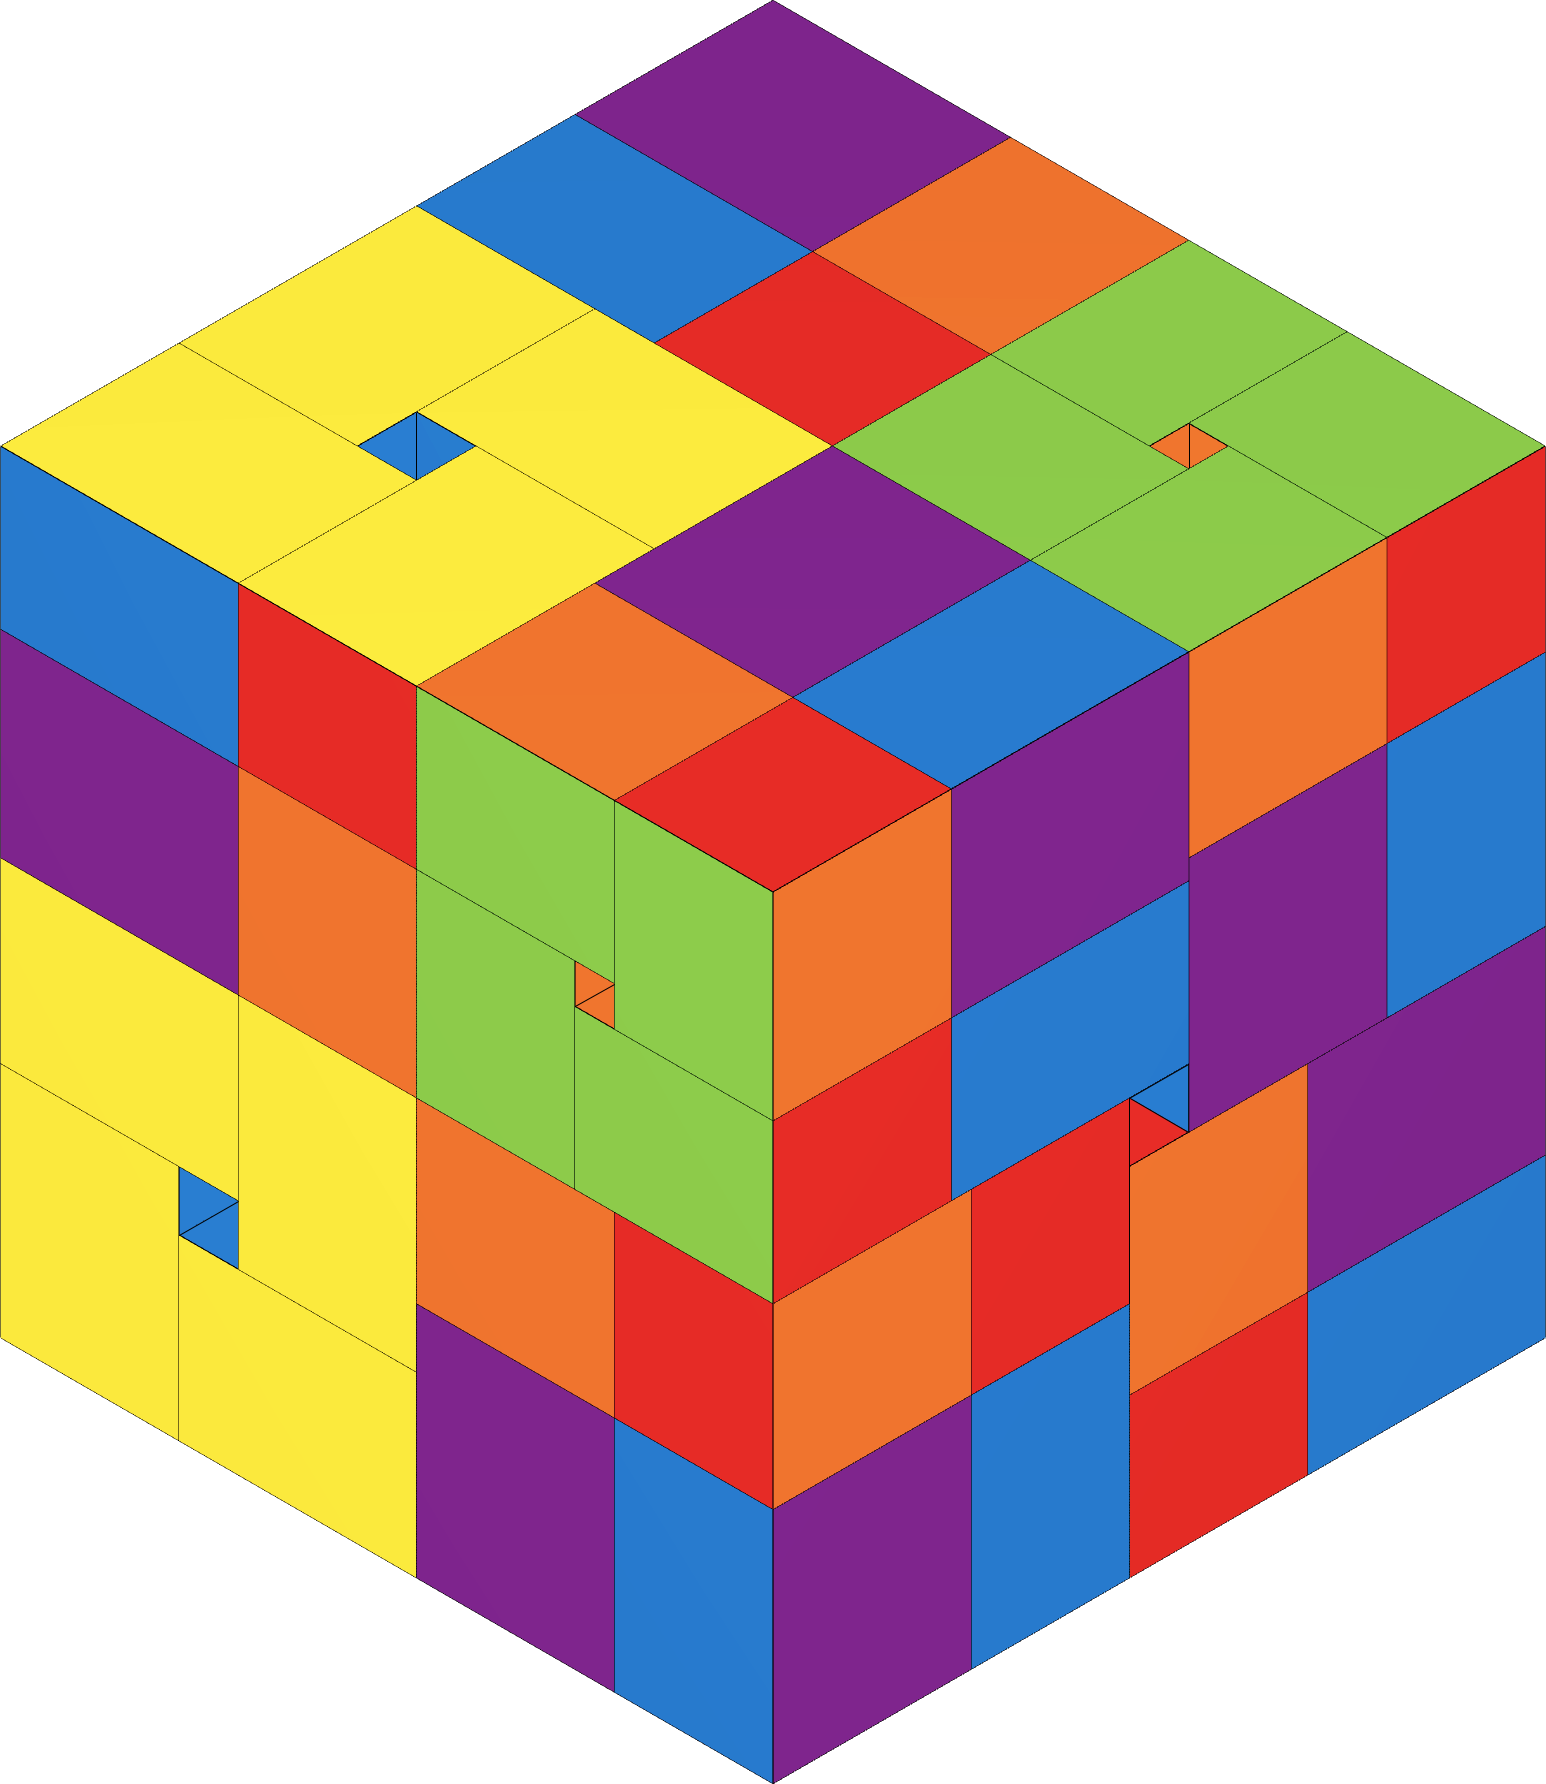
\includegraphics[scale=0.18]{graphics/4d-universal-cube-1.png}
        \caption*{$x = 1$.}
    \end{subfigure}
    ~
    \begin{subfigure}[b]{0.47\textwidth}
        \centering
        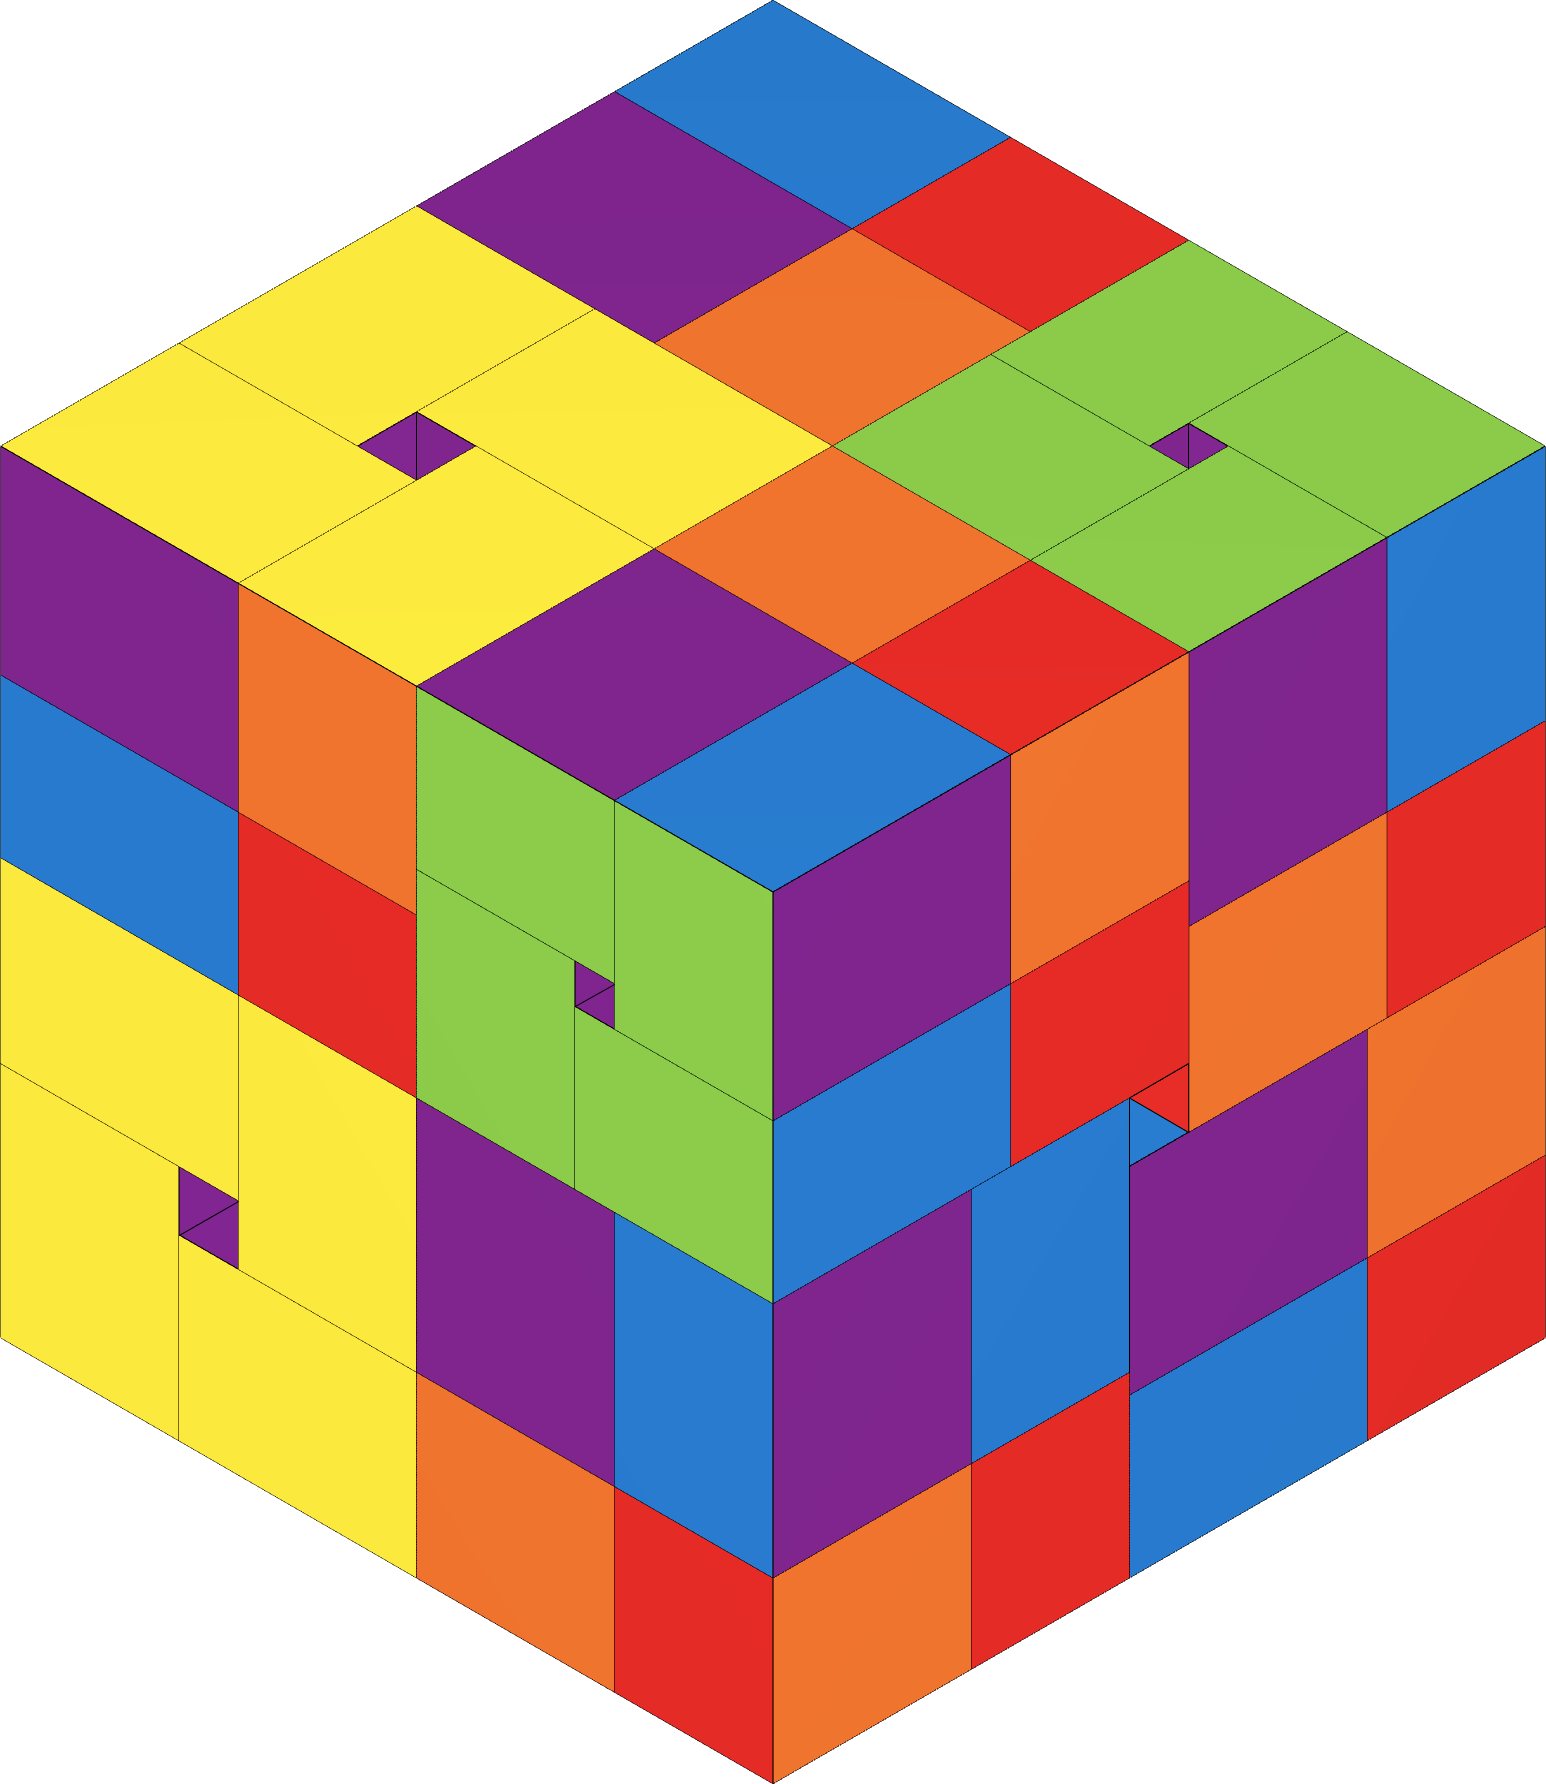
\includegraphics[scale=0.18]{graphics/4d-universal-cube-2.png}
        \caption*{$x = 2$.}
    \end{subfigure}
    \par\bigskip
    \begin{subfigure}[b]{0.47\textwidth}
        \centering
        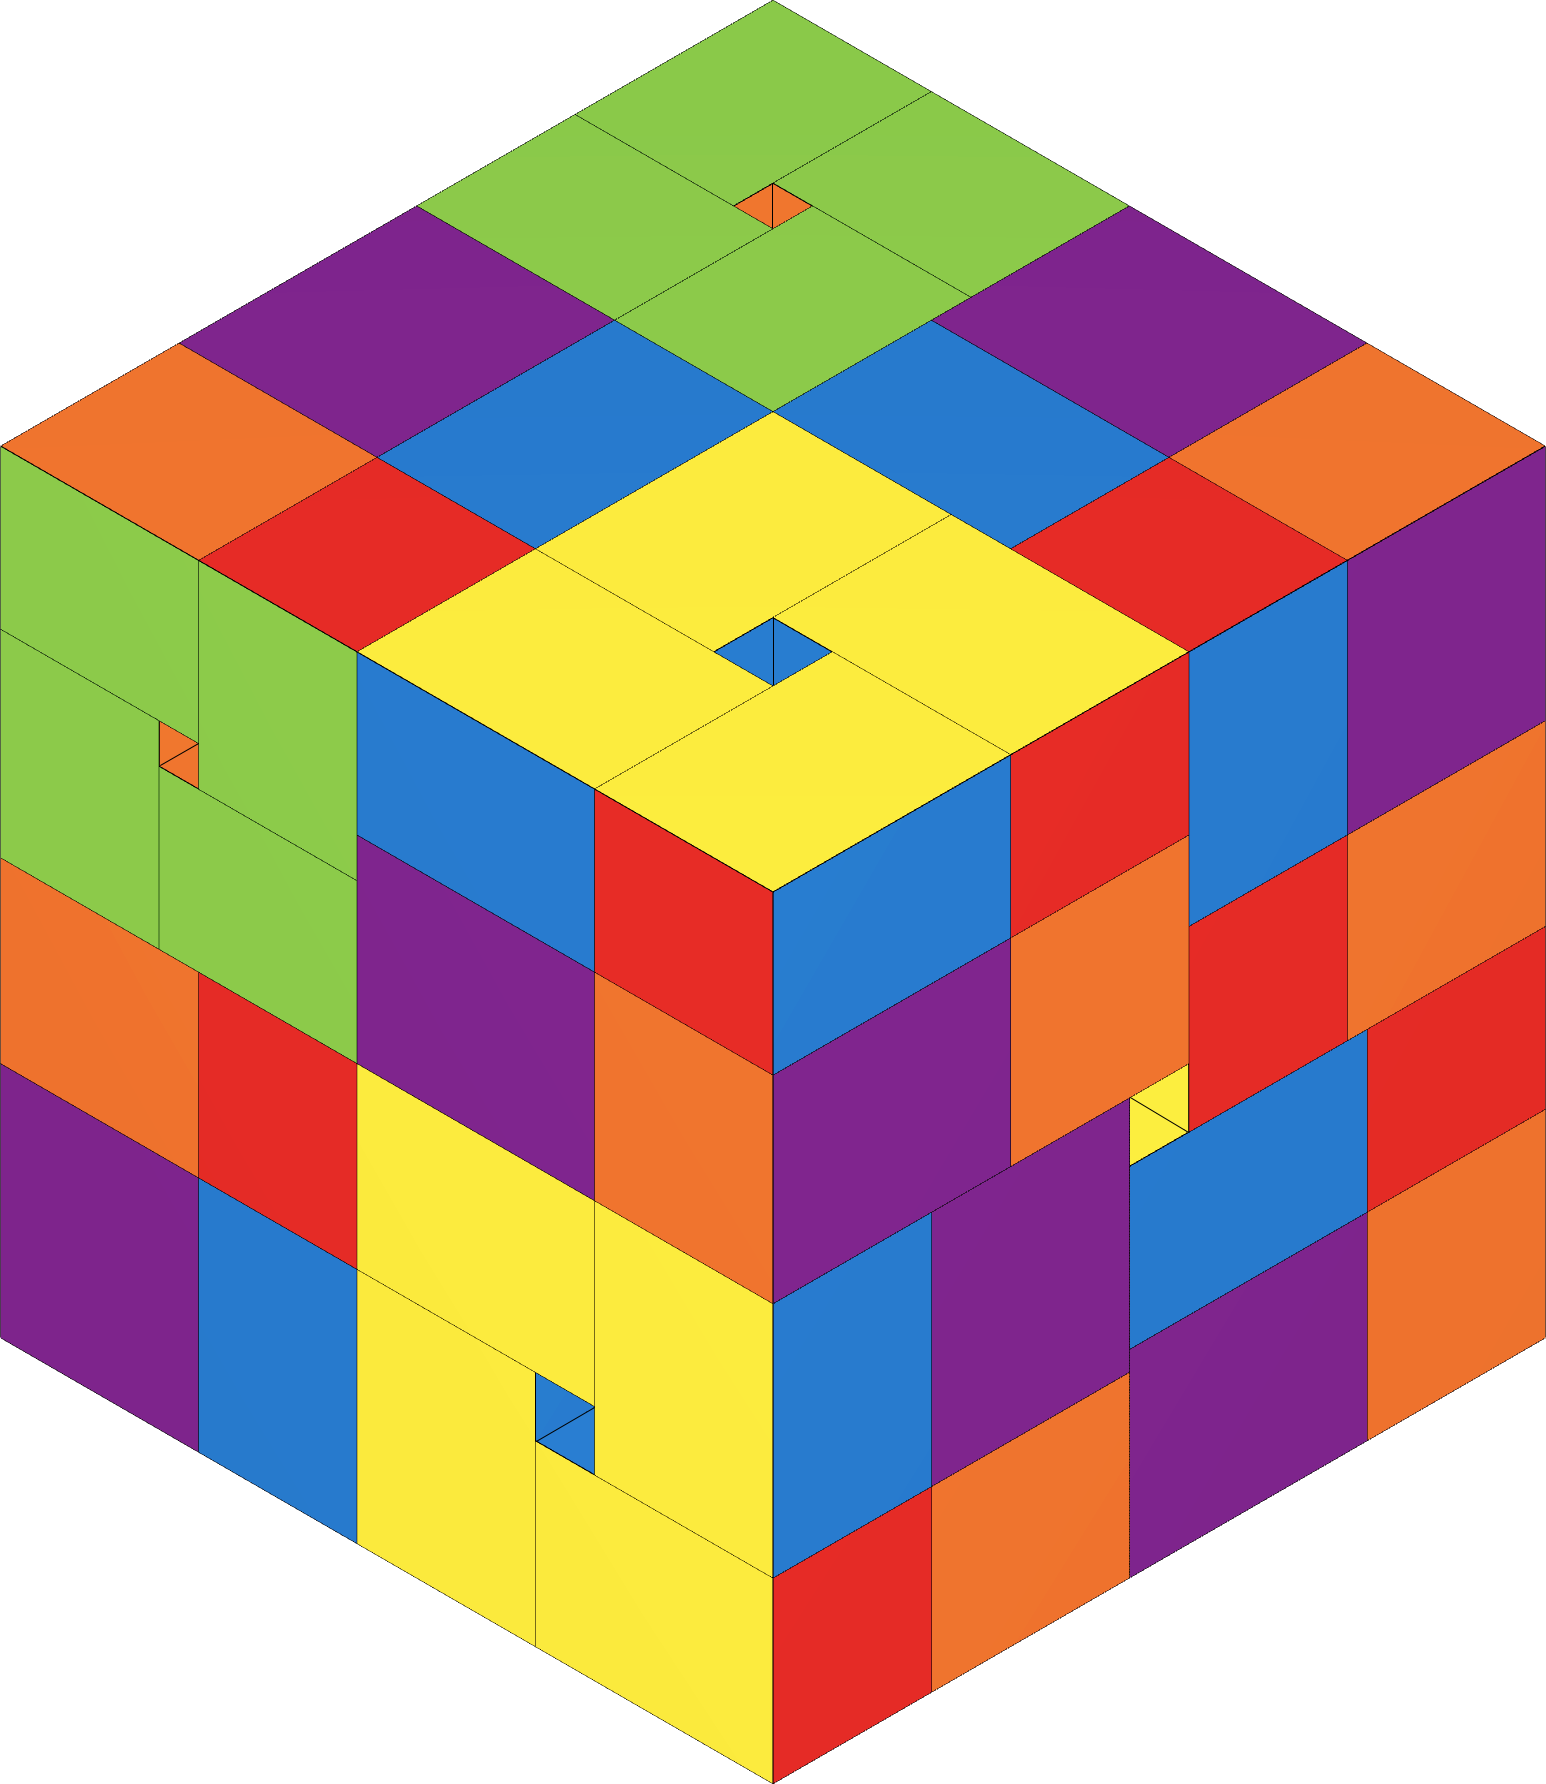
\includegraphics[scale=0.18]{graphics/4d-universal-cube-3.png}
        \caption*{$x = 3$.}
    \end{subfigure}
    ~
    \begin{subfigure}[b]{0.47\textwidth}
        \centering
        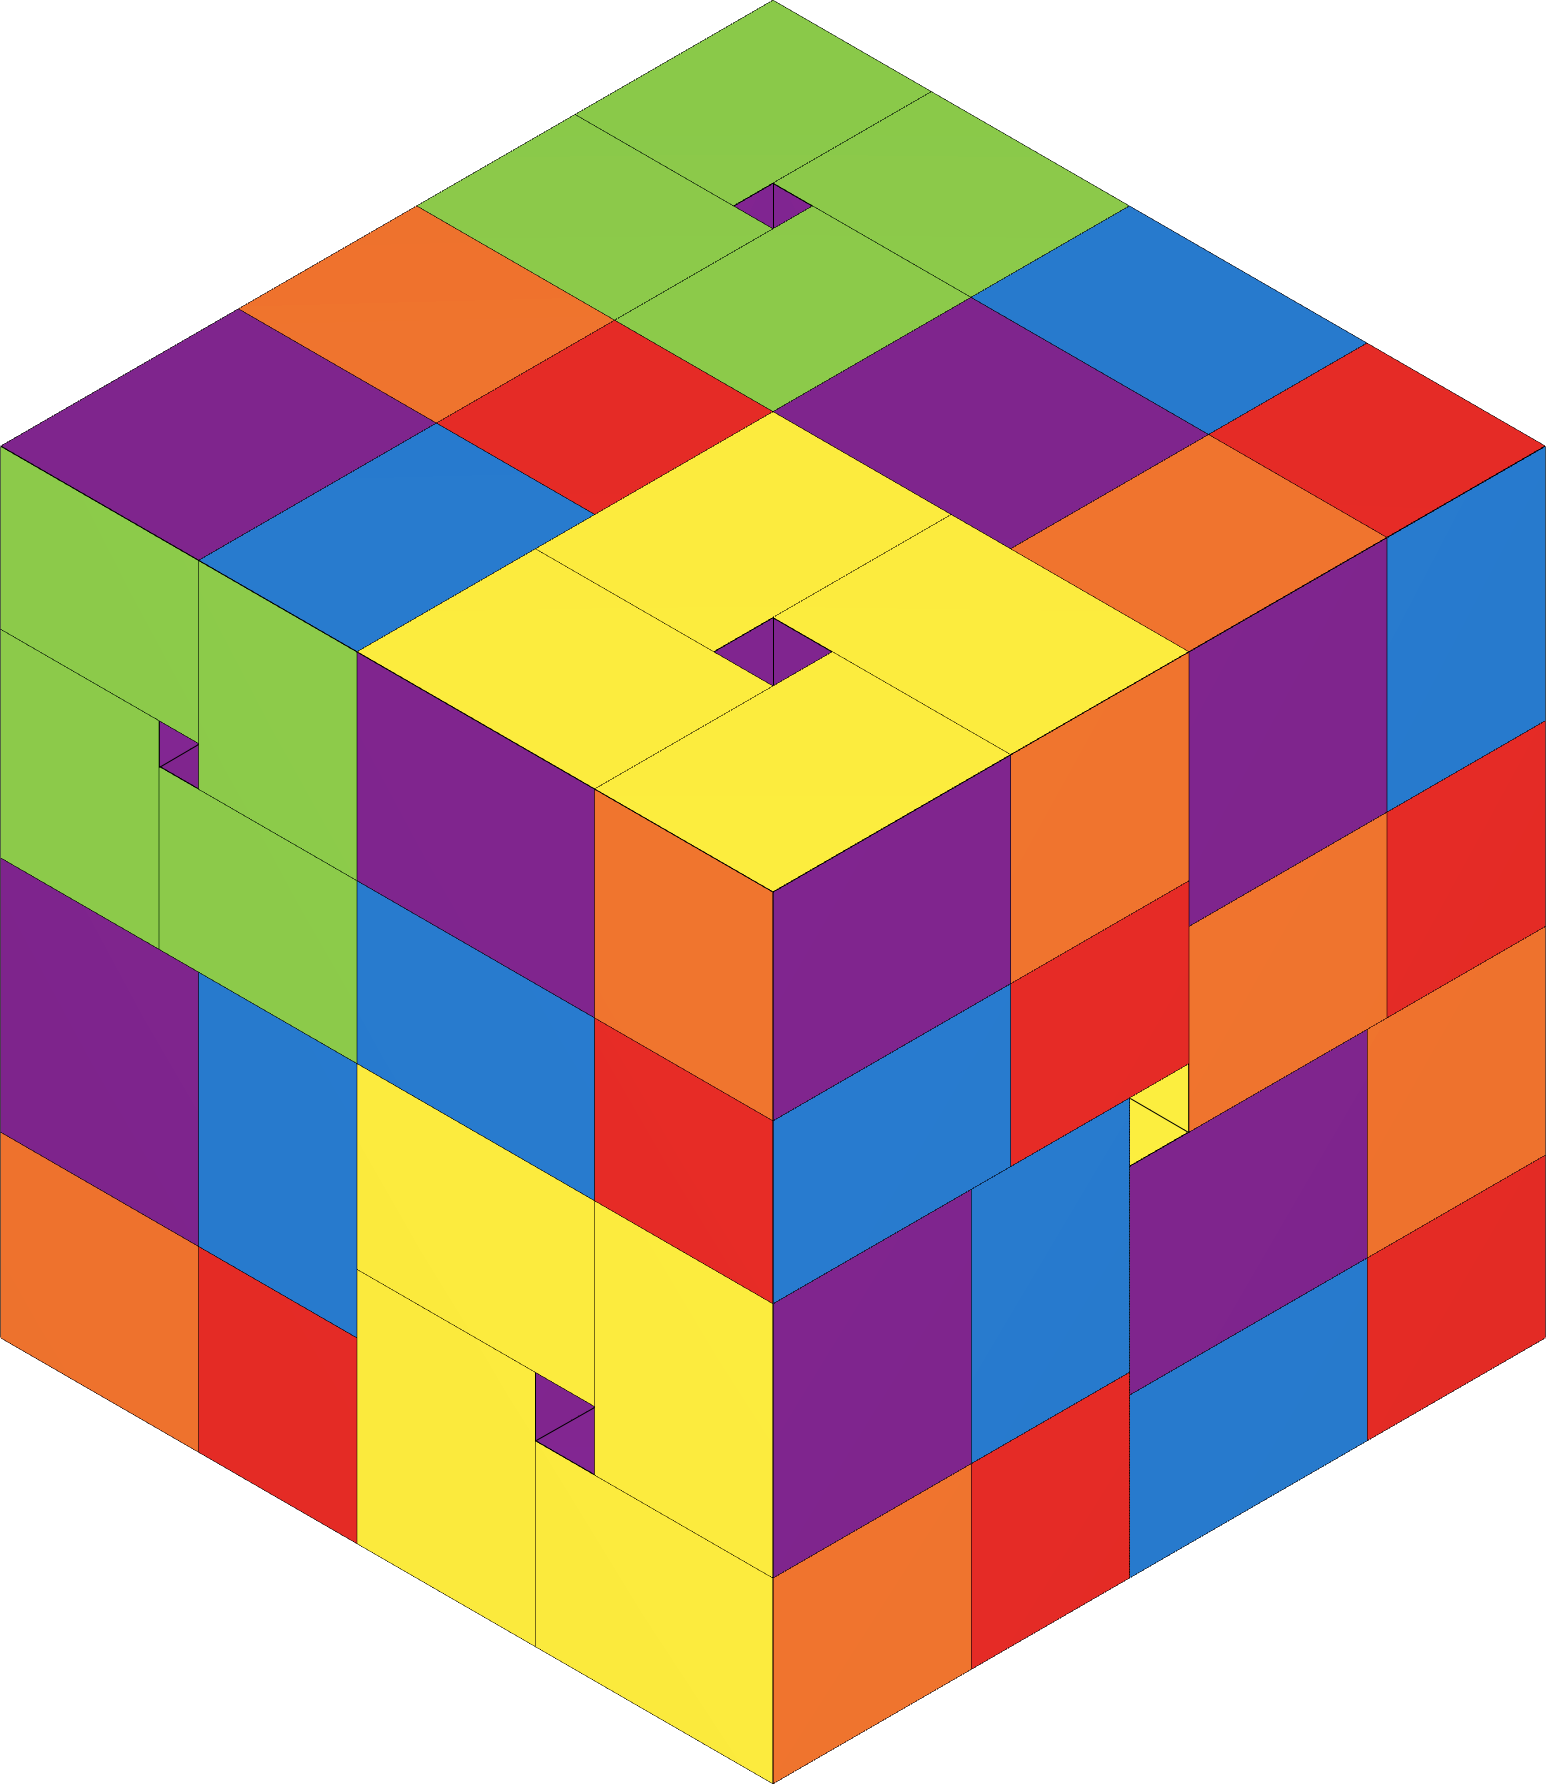
\includegraphics[scale=0.18]{graphics/4d-universal-cube-4.png}
        \caption*{$x = 4$.}
    \end{subfigure}
    \caption{Visualization of the four cubes of a four-dimensional universal packing where the $x$-axis is fixed. The packing has been produced using the dimension tuple $\paren{8, 9, 10, 12}$.}
    \label{fig:4d-universal-packing}
\end{figure}

\noindent These universal packings behave extremely nice.

\begin{observation}
Notice that the two-dimensional packing in \cref{fig:universal-packing-2d} is stable under any permutation from $S_2$. We have examined whether the universal packings constructed in \cref{obs:combined-4d} are stable under permutations from $S_4$. It turns out that they are stable under any permutation from $S_4$. We speculate that this property is inherited through the proof of \cref{thm:multiplication-of-packings}. It is dubious whether all four-dimensional universal packings exhibit this property. It is worth noting that this investigation also resulted in the universal packing from which \cref{fig:4d-square-universal} originates and thus sparked the investigation into a RDTS.
\end{observation}

\subsection{The subgrid criterion}
The four-dimensional universal packings constructed in \cref{obs:combined-4d} provided the inspiration for how to generalize the last major piece of knowledge provided by Hoffman in \cite[p. 221]{Hoffman1981} about the three-dimensional problem. Let $(x_1, x_2, x_3)$ be an increasing dimension tuple with distinct elements. Consider a square of it produced by a three-dimensional universal packing. Such a square contains $3^2 = 9$ rectangles, and Hoffman notes that these $9$ rectangles must comprise exactly 3 $x_1$-by-$x_2$'s, $x_1$-by-$x_3$'s and $x_2$-by-$x_3$'s. This is illustrated in \cref{fig:universal-packing-3d} where each type of rectangle has been given its own color. This observation has proven to be effective at pruning the search tree as seen in \cref{fig:backtracking-3d} and \cref{table:backtracking-3d}. Hence, we have had a great interest in generalizing this observation to higher dimensions in the hope that it will be similarly effective there.

\begin{observation}
The following is the case for any of the universal packings constructed in \cref{obs:combined-4d}. Let $(x_1, x_2, x_3, x_4)$ denote the dimension tuple with distinct elements, which has been used. Consider some cube of $G_4$ and note that it produces a subpacking containing $4^3 = 64$ bricks. These 64 bricks comprise exactly 16 $x_1$-by-$x_2$-by-$x_3$'s, $x_1$-by-$x_2$-by-$x_4$'s, $x_1$-by-$x_3$-by-$x_4$'s and $x_2$-by-$x_3$-by-$x_4$'s.
\end{observation}

\noindent This provides enough information to put forward the following criterion.

\begin{criterion}[Subgrid criterion]\label[criterion]{criterion:subgrid-criterion}\index{Criterion!subgrid}
Suppose $n \geq 2$ and suppose $P\colon G_n \to S_n$. We say that $P$ satisfies the \textit{Subgrid criterion} if any $\paren{n - 1}$-dimensional subgrid $U$ of $G_n$ satisfies the following: Suppose $d = \paren{x_1, x_2, \dotsc, x_n}$ is an increasing dimension tuple with distinct elements and consider the subpacking produced by $P$ restricted to $U$. This subpacking (consisting of $n^{n - 1}$ $\paren{n - 1}$-dimensional hyperrectangles) contains precisely $n^{n - 2}$ hyperrectangles without an extent of $x_i$ for all $i = 1, 2, \dotsc, n$.
\end{criterion}

\noindent Even better, we have been able to prove that this is a necessary condition for being a universal packing.

\begin{proposition}
Suppose $n \geq 2$ and suppose $P\colon G_n \to S_n$ is a universal packing. Then $P$ satisfies the Subgrid criterion \labelcref{criterion:subgrid-criterion}.
\end{proposition}

\begin{proof}
Note that $P$ satisfies the Line criterion \labelcref{criterion:line-criterion} by \cref{prop:universal-packing-has-unique-lines}. Take some $\paren{n - 1}$-dimensional subgrid $U$ of $G_n$ and consider the subpacking produced by $P$ restricted to $U$. There are $(n - 1)n^{n - 2}$ grid lines in $U$, since there are $n^{n - 2}$ grid lines along each of the $n - 1$ different dimensions. Take some $i$ in $\curly{1, 2, \dotsc, n}$. For each of these grid lines there must be precisely one hyperrectangle on it with an extent of $x_i$ along the dimension of the grid line. Hence, there are at least $(n - 1)n^{n - 2}$ hyperrectangles in the subpacking with an extent of $x_i$ along some dimension. Notice that the subpacking consists of $n^{n - 1}$ $\paren{n - 1}$-dimensional hyperrectangles with a total number of $(n - 1)n^{n - 1}$ extends. Since $i$ was chosen arbitrarily, it follows that there must be precisely $(n - 1)n^{n - 2}$ hyperrectangles in the subpacking with an extent of $x_i$ along some dimension. Then the subpacking consists of precisely
\[
n^{n - 1} - (n - 1)n^{n - 2} = n^{n - 2}
\]
$\paren{n - 1}$-dimensional hyperrectangles without an extent of $x_i$. Hence, $P$ satisfies the Subgrid criterion \labelcref{criterion:subgrid-criterion}.
\end{proof}

\begin{example}
Suppose we have a packing produced by a universal packing. In the three-dimensional case we can conclude that there will be $3^{3 - 2} = 3$ of each of the 3 different types of rectangles in each square. In the four-dimensional case we can conclude that there must be $4^{4 - 2} = 16$ of each of the 4 different types of bricks in each cube.
\end{example}

\noindent In \cite{Hoffman1981} Hoffman puts great emphasis on the close relationship between inequalities and packing problems and the Subgrid criterion does also have an interesting interpretation as an inequality.

\begin{corollary}
Suppose $n \geq 2$ and suppose there exists a universal packing $P\colon G_n \to S_n$. Then for any dimension tuple $d = \paren{x_1, x_2, \dotsc, x_n}$ satisfying Hoffman's inequality, we have that
\[
n^{n-2}\paren{\sum_{i=1}^{n}{\frac{1}{x_i}}} \paren{\prod_{i=1}^{n}{x_i} }
\leq \paren{\sum_{i=1}^{n}{x_i}}^{n-1}.
\]
\end{corollary}

\begin{proof}
Take some $\paren{n - 1}$-dimensional subgrid $U$ of $G_n$ and consider the subpacking of $d$ produced by $P$ restricted to $U$. Pick some $j$ in $\curly{1, 2, \dotsc, n}$ and let us determine the combined hypervolume of the hyperrectangles without an extent of $x_j$. By the Subgrid criterion \labelcref{criterion:subgrid-criterion} there are $n^{n - 2}$ of these hyperrectangles yielding a combined hypervolume of
\[
\frac{n^{n - 2}}{x_j}\prod_{i = 1}^{n}{x_i}.
\]
Then the combined hypervolume of all of the hyperrectangles in the subpacking is
\[
n^{n-2}\paren{\sum_{i=1}^{n}{\frac{1}{x_i}}} \paren{\prod_{i=1}^{n}{x_i}}.
\]
Notice that the surrounding $\paren{n - 1}$-dimensional hypercube has an extent of $x_1 + x_2 + \dotsb + x_n$ and hence a hypervolume of $\paren{x_1 + x_2 + \dotsb + x_n}^{n - 1}$. All of the $\paren{n - 1}$-dimensional hyperrectangles are pairwise non-overlapping and contained inside the surrounding $\paren{n - 1}$-dimensional hypercube. Hence, the inequality holds.
\end{proof}

\noindent This is interesting, since if the above inequality does not hold in general, then it might be possible to rule out the existence of a Hoffman packing for certain dimension tuples and perhaps even show that a dimension is not good. However, it turns out that this inequality does in fact hold in general, since it follows quite easily \cite{Martin2017} from Maclaurin's inequality \cite[p. 188]{Cvetkovski2012}. For $n = 4$, Maclaurin's inequality states that
\begin{align}
\frac{x_1 + x_2 + x_3 + x_4}{4}
&\ge \sqrt{\frac{x_1x_2 + x_1x_3 + x_1x_4 + x_2x_3 + x_2x_4 + x_3x_4}{6}}\label{eq:4d-mac-2d}\\
&\ge \sqrt[3]{\frac{x_1x_2x_3 + x_1x_2x_4 + x_1x_3x_4 + x_2x_3x_4}{4}}\label{eq:4d-mac-3d}\\
&\ge \sqrt[4]{x_1x_2x_3x_4}.\label{eq:4d-mac-4d}
\end{align}
for any positive real numbers $x_1, x_2, x_3$ and $x_4$. The inequality given by the left-hand side of \eqref{eq:4d-mac-2d} combined with \eqref{eq:4d-mac-4d} expresses the AM-GM inequality, while the inequality given by the left-hand side of \eqref{eq:4d-mac-2d} combined with \eqref{eq:4d-mac-3d} expresses the inequality treated above for $n = 4$. Inspired by Hoffman's focus on the close relationship between inequalities and packing problems let us see if we can find a connection between \eqref{eq:4d-mac-2d} and the four-dimensional problem. This inequality can be rearranged to
\begin{equation}\label{eq:4d-mac-2d-six-squares}
16\paren{x_1x_2 + x_1x_3 + x_1x_4 + x_2x_3 + x_2x_4 + x_3x_4}
\leq 6\paren{x_1 + x_2 + x_3 + x_4}^2
\end{equation}
or equivalently
\begin{equation}\label{eq:4d-mac-2d-three-squares}
8\paren{x_1x_2 + x_1x_3 + x_1x_4 + x_2x_3 + x_2x_4 + x_3x_4}
\leq 3\paren{x_1 + x_2 + x_3 + x_4}^2,
\end{equation}
and the power of two on the right-hand side motivates us to look for a connection among the squares.

\begin{observation}\label[observation]{obs:4d-n-2-subgrid}
The following is the case for any of the universal packings constructed in \cref{obs:combined-4d}. Let $(x_1, x_2, x_3, x_4)$ denote the dimension tuple with distinct elements, which has been used. Take any 3 pairwise ``orthogonal'' squares and consider the $3 \cdot 4^2 = 48$ rectangles in them. These 48 rectangles comprise exactly 8 $x_1$-by-$x_2$'s, $x_1$-by-$x_3$'s, $x_1$-by-$x_4$'s, $x_2$-by-$x_3$'s, $x_2$-by-$x_4$'s and $x_3$-by-$x_4$'s. The phenomenon can be observed in \cref{fig:4d-universal-packing} and all the squares of this packing can be found in \cref{appendix-B}. Notice that this implies that ``parallel'' squares have the same number of each type of rectangle.
\end{observation}

\noindent This corresponds precisely to the inequality \eqref{eq:4d-mac-2d-three-squares}. It has not been possible to prove that this is a necessary condition for being a universal packing. Neither has it been possible to come up with a counterexample. Even if this is not the case, a weaker claim might still hold, namely that there are 16 of each type of rectangle in any six pairwise ``orthogonal'' squares. This corresponds to the inequality \eqref{eq:4d-mac-2d-six-squares}.

In order to come up with a counterexample or strengthen the above two hypotheses, we need another way of constructing a four-dimensional universal packing. Since the ordinary backtracking and dynamic programming approaches does not show much promise, we have also tried an alternative approach.

\begin{observation}
Starting from one of the universal packings constructed in \cref{obs:combined-4d}, we removed a number of hyperrectangles and then attempted to use backtracking to complete this partial solution. We could remove up to 94 hyperrectangles without completely derailing the backtracking algorithm. Without terminating after two days it had found $C = 435\,122\,478$ universal packings. A few random samples of these did not provide a counterexample to any of the two hypotheses above. These solutions appear to have the same overall structure as the universal packings from \cref{obs:combined-4d}, but with some of the hyperrectangles swapped around. This is illustrated in \cref{fig:4d-partial-swaps}. Since any unique four-dimensional universal packing has at most $4! \cdot 2^4 = 384$ non-coinciding symmetries by \cref{prop:universal-symmetries} there must be at least $\floor*{C/384} = 1\,133\,131$ unique universal packings in the four-dimensional case.
\end{observation}

\begin{figure}[ht]
    \centering
    \begin{subfigure}[b]{0.220\textwidth}
        \centering
        \begin{tikzpicture}[scale=0.068]
\filldraw[fill=custom-blue, draw=black] (0,0) rectangle (8,12);
\filldraw[fill=custom-red, draw=black] (0,12) rectangle (8,21);
\filldraw[fill=custom-red, draw=black] (0,21) rectangle (9,29);
\filldraw[fill=custom-orange, draw=black] (0,29) rectangle (9,39);
\filldraw[fill=custom-violet, draw=black] (8,0) rectangle (18,12);
\filldraw[fill=custom-orange, draw=black] (8,12) rectangle (18,21);
\filldraw[fill=custom-blue, draw=black] (9,21) rectangle (21,29);
\filldraw[fill=custom-violet, draw=black] (9,29) rectangle (21,39);
\filldraw[fill=custom-blue, draw=black] (18,0) rectangle (30,8);
\filldraw[fill=custom-violet, draw=black] (18,8) rectangle (30,18);
\filldraw[fill=custom-blue, draw=black] (21,18) rectangle (29,30);
\filldraw[fill=custom-red, draw=black] (21,30) rectangle (29,39);
\filldraw[fill=custom-red, draw=black] (30,0) rectangle (39,8);
\filldraw[fill=custom-orange, draw=black] (30,8) rectangle (39,18);
\filldraw[fill=custom-violet, draw=black] (29,18) rectangle (39,30);
\filldraw[fill=custom-orange, draw=black] (29,30) rectangle (39,39);
        \end{tikzpicture}
    \end{subfigure}
    ~
    \begin{subfigure}[b]{0.220\textwidth}
        \centering
        \begin{tikzpicture}[scale=0.068]
\filldraw[fill=custom-blue, draw=black] (0,0) rectangle (8,12);
\filldraw[fill=custom-red, draw=black] (0,12) rectangle (8,21);
\filldraw[fill=custom-blue, draw=black] (0,21) rectangle (12,29);
\filldraw[fill=custom-orange, draw=black] (0,29) rectangle (9,39);
\filldraw[fill=custom-orange, draw=black] (8,0) rectangle (18,9);
\filldraw[fill=custom-violet, draw=black] (8,9) rectangle (18,21);
\filldraw[fill=custom-red, draw=black] (12,21) rectangle (21,29);
\filldraw[fill=custom-violet, draw=black] (9,29) rectangle (21,39);
\filldraw[fill=custom-blue, draw=black] (18,0) rectangle (30,8);
\filldraw[fill=custom-violet, draw=black] (18,8) rectangle (30,18);
\filldraw[fill=custom-blue, draw=black] (21,18) rectangle (29,30);
\filldraw[fill=custom-red, draw=black] (21,30) rectangle (29,39);
\filldraw[fill=custom-red, draw=black] (30,0) rectangle (39,8);
\filldraw[fill=custom-orange, draw=black] (30,8) rectangle (39,18);
\filldraw[fill=custom-violet, draw=black] (29,18) rectangle (39,30);
\filldraw[fill=custom-orange, draw=black] (29,30) rectangle (39,39);
        \end{tikzpicture}
    \end{subfigure}
    ~
    \begin{subfigure}[b]{0.220\textwidth}
        \centering
        \begin{tikzpicture}[scale=0.068]
\filldraw[fill=custom-blue, draw=black] (0,0) rectangle (8,12);
\filldraw[fill=custom-red, draw=black] (0,12) rectangle (8,21);
\filldraw[fill=custom-blue, draw=black] (0,21) rectangle (12,29);
\filldraw[fill=custom-violet, draw=black] (0,29) rectangle (12,39);
\filldraw[fill=custom-orange, draw=black] (8,0) rectangle (18,9);
\filldraw[fill=custom-violet, draw=black] (8,9) rectangle (18,21);
\filldraw[fill=custom-red, draw=black] (12,21) rectangle (21,29);
\filldraw[fill=custom-orange, draw=black] (12,29) rectangle (21,39);
\filldraw[fill=custom-red, draw=black] (18,0) rectangle (27,8);
\filldraw[fill=custom-violet, draw=black] (18,8) rectangle (30,18);
\filldraw[fill=custom-blue, draw=black] (21,18) rectangle (29,30);
\filldraw[fill=custom-red, draw=black] (21,30) rectangle (29,39);
\filldraw[fill=custom-blue, draw=black] (27,0) rectangle (39,8);
\filldraw[fill=custom-orange, draw=black] (30,8) rectangle (39,18);
\filldraw[fill=custom-violet, draw=black] (29,18) rectangle (39,30);
\filldraw[fill=custom-orange, draw=black] (29,30) rectangle (39,39);
        \end{tikzpicture}
    \end{subfigure}
    ~
    \begin{subfigure}[b]{0.220\textwidth}
        \centering
        \begin{tikzpicture}[scale=0.068]
\filldraw[fill=custom-blue, draw=black] (0,0) rectangle (8,12);
\filldraw[fill=custom-red, draw=black] (0,12) rectangle (8,21);
\filldraw[fill=custom-blue, draw=black] (0,21) rectangle (12,29);
\filldraw[fill=custom-orange, draw=black] (0,29) rectangle (9,39);
\filldraw[fill=custom-orange, draw=black] (8,0) rectangle (18,9);
\filldraw[fill=custom-violet, draw=black] (8,9) rectangle (18,21);
\filldraw[fill=custom-red, draw=black] (12,21) rectangle (21,29);
\filldraw[fill=custom-violet, draw=black] (9,29) rectangle (21,39);
\filldraw[fill=custom-red, draw=black] (18,0) rectangle (27,8);
\filldraw[fill=custom-violet, draw=black] (18,8) rectangle (30,18);
\filldraw[fill=custom-blue, draw=black] (21,18) rectangle (29,30);
\filldraw[fill=custom-red, draw=black] (21,30) rectangle (29,39);
\filldraw[fill=custom-blue, draw=black] (27,0) rectangle (39,8);
\filldraw[fill=custom-orange, draw=black] (30,8) rectangle (39,18);
\filldraw[fill=custom-violet, draw=black] (29,18) rectangle (39,30);
\filldraw[fill=custom-orange, draw=black] (29,30) rectangle (39,39);
        \end{tikzpicture}
    \end{subfigure}
    \caption{Example of how completing a partial solution in multiple ways might lead to a swapping of some of the hyperrectangles.}
    \label{fig:4d-partial-swaps}
\end{figure}


\noindent This observation indicates that some regions of the search space might have a particularly high density of solutions and also that there are a \textit{lot} of four-dimensional unique universal packings compared to the three-dimensional case.
